\documentclass[11pt,letterpaper]{article}
\usepackage[margin=0.83in,includefoot]{geometry}
\usepackage[T1]{fontenc}
\usepackage{lmodern}
\usepackage{amsmath,amssymb,graphicx,booktabs,siunitx,microtype}
\usepackage[font=small,labelfont=bf]{caption}
\usepackage{float,placeins}
\usepackage[hidelinks]{hyperref}
\hypersetup{pdftitle={Linear Gyrokinetic Stability of Dipole-Confined Plasmas: Phase 1 and Phase 2 Research Results},pdfauthor={MAE 190 Research Project}}
\graphicspath{{figures/}}
\setlength{\parindent}{0pt}
\setlength{\parskip}{5pt plus 1pt}
\setlength{\textfloatsep}{13pt plus 3pt minus 2pt}
\setlength{\intextsep}{12pt plus 3pt minus 2pt}
\renewcommand{\topfraction}{.91}
\renewcommand{\bottomfraction}{.75}
\renewcommand{\textfraction}{.10}
\renewcommand{\floatpagefraction}{.76}
\newcommand{\omn}{\mathrm{omn}}
\newcommand{\omt}{\mathrm{omt}}
\newcommand{\kn}{k_y\rho_{\rm ref}}
\newcommand{\gr}{\widehat\gamma}
\newcommand{\fr}{\widehat\omega}
\newcommand{\ttime}{\widehat t}
\newcommand{\studyfig}[3]{\begin{figure}[!htbp]\centering\includegraphics[width=\linewidth]{#1.pdf}\caption{#3}\label{#2}\end{figure}}
\title{Linear Gyrokinetic Stability of Dipole-Confined Plasmas:\\[4pt] Phase 1 and Phase 2 Research Results}
\author{MAE 190 Research Project}
\date{Revised November 19, 2026}

\newcommand{\matrixrows}{%
1 & 0.5 & 3.451 & $+0.434$ & $24\times48\times24$ \\
1 & 0.7 & 3.294 & $+0.591$ & $24\times48\times24$ \\
1 & 1 & 2.974 & $+0.795$ & $24\times48\times24$ \\
1 & 1.5 & 2.273 & $+1.044$ & $24\times48\times24$ \\
2 & 0.5 & 4.309 & $+0.685$ & $32\times48\times32$ \\
2 & 0.7 & 4.179 & $+0.947$ & $24\times48\times24$ \\
2 & 1 & 3.900 & $+1.314$ & $32\times48\times32$ \\
2 & 1.5 & 3.339 & $+1.839$ & $32\times48\times32$ \\
2 & 2 & 2.799 & $+2.275$ & $32\times48\times32$ \\
3 & 0.5 & 5.015 & $+0.934$ & $24\times48\times24$ \\
3 & 0.7 & 4.868 & $+1.296$ & $24\times48\times24$ \\
3 & 1 & 4.570 & $+1.819$ & $24\times48\times24$ \\
3 & 1.5 & 3.933 & $+2.625$ & $24\times48\times24$ \\%
}

\newcommand{\energyfitrows}{%
Hydrogen & 0 & 0 & $-0.0801$ & $-0.0867$ & $-0.0814$ & Qualified \\
Hydrogen & 0 & 0.5 & $-0.1534$ & $-0.0682$ & $-0.0658$ & Uncertain \\
Hydrogen & 0 & 1 & $+1.2817$ & $+0.9119$ & $+0.4963$ & Uncertain \\
Hydrogen & 0.5 & 0 & $+0.2423$ & $+0.1170$ & $+0.0901$ & Uncertain \\
Hydrogen & 0.5 & 0.5 & $+0.1467$ & $+0.2137$ & $+0.4583$ & Uncertain \\
Deuterium & 0 & 0 & $-0.0621$ & $-0.0610$ & $-0.0750$ & Qualified \\
Deuterium & 0 & 0.5 & $-0.0457$ & $-0.1621$ & $-0.2419$ & Uncertain \\
Deuterium & 0 & 1 & $+0.9176$ & $+1.2254$ & $+1.0064$ & Uncertain \\
Deuterium & 0 & 2 & $+1.7597$ & $+1.7101$ & $+1.6826$ & Qualified \\
Deuterium & 0.5 & 0 & $+0.2268$ & $+0.2920$ & $+0.2612$ & Qualified \\
Deuterium & 0.5 & 0.5 & $+0.0833$ & $+0.0464$ & $+0.0880$ & Uncertain \\
Deuterium & 0.5 & 1 & $+1.2265$ & $+1.1691$ & $+1.1351$ & Qualified \\
Deuterium & 1 & 0 & $+1.0653$ & $+1.0783$ & $+1.0837$ & Qualified \\%
}

\newcommand{\FollowupAbstract}{A charge-balanced helium pilot demonstrates a feasible electron-gradient path at fixed deuterium gradient. At low wavenumber, two half-step controls replace the historical grid-scale runaway and aliased frequency with a repeatable moderately growing mode.}
\newcommand{\HeliumResult}{All three IV points at $\kn=0.7$ and grid $24\times48\times24$ converged without rescaling. Growth increased from 3.905 through 4.067 to 4.221, and real frequency increased from $+0.733$ through $+0.768$ to $+0.805$ (Fig.~\ref{fig:helium}). The projected late-time slopes agree with the native values. Each outer final complex profile overlaps the midpoint by more than 0.9999992, consistent with a similar dominant mode along this narrow path.}
\newcommand{\LowKyResult}{The original automatic run at $\kn=0.3$ amplified a grid-scale signal and returned an aliased real frequency. Both half-step controls converge to a smooth growing mode with $\gr\simeq4.40$ and $\fr=+0.415$. This supports a timestep-sensitive numerical origin for the historical extreme rates. The original value is excluded. The qualified $0.3$ result at common $\omn=2$ is slightly larger in growth than the neighboring 0.5 point. Appendix~\ref{app:lowky} gives the comparison and alias reconstruction.}
\newcommand{\LowKyDetails}{Both fixed-step controls used $\Delta\ttime=0.0004175$ and the original velocity-space grids and collision operator. They converged without rescaling. On the shared late interval $1.659\leq\ttime\leq2.158$, the fitted growth rates differ by 0.123\% and the real frequencies by 0.022\% relative to 32 points. The final complex overlap is 0.999999996 across the two grids and about 0.99993 with the qualified $\kn=0.5$ profile. The two runs therefore support a repeatable physical-scale IV mode at $0.3$. The original automatic step was near the RKC2 collisional restriction, and the fixed setup retains two collision evaluations per step with a supplied bound. We can identify a timestep-sensitive numerical instability and a frequency alias without assigning the runaway to a specific term of the discrete operator.}
\newcommand{\LowKyRows}{%
Original automatic & 32 & 0.0008350 & 3129 & 378.519 & $+220.647$ & 29 \\
Fixed step & 32 & 0.0004175 & 5529 & 4.403 & $+0.415$ & 0 \\
Fixed step, refined & 48 & 0.0004175 & 5169 & 4.398 & $+0.415$ & 0 \\
}


\begin{document}
\maketitle
\begin{abstract}
Small electrostatic disturbances in a magnetic dipole can grow and rotate at different rates. We used linear gyrokinetic initial-value calculations to identify how density gradients, wavelength, ion mass and the electron response affect these rates. The historical studies establish a growing electron--positron mode with stationary phase and faster growth in hydrogen than deuterium at all 41 qualified matched gradient points. In the density-focused deuterium study, steeper common gradients increase growth and real frequency. Shorter sampled binormal wavelengths reduce growth over the established $0.5\leq\kn\leq1.5$ interval. Replacing kinetic electrons by a Boltzmann response at one collisionless point reduces growth by 96.7\% and reverses the sign of the real frequency. \FollowupAbstract
\end{abstract}

\section{Physical question and model}
A magnetic dipole bends field lines into closed loops. Particles travel along and drift across the lines; some are reflected where the field strengthens. Equilibrium density and temperature gradients supply free energy for small disturbances. In this paper, \emph{growth} means increasing amplitude of an electrostatic potential perturbation, and \emph{real frequency} measures the rotation of its Fourier phase. Linear growth indicates an instability of the modeled equilibrium. Nonlinear saturation, transport and experimental confinement require separate evidence.

GENE evolves a gyrokinetic distribution and solves for its self-consistent fields \cite{jenko2000,goerler2011}. Gyrokinetics averages over fast gyromotion while retaining the orbit and velocity-space dynamics relevant to the lower-frequency perturbation. We use the local, electrostatic initial-value path (\texttt{comp\_type = 'IV'}), one radial and one nonzero binormal mode, and periodic parallel boundaries in the ring dipole. The imposed ring radius is \SI{0.4}{\meter}, current \SI{750}{\ampere}, and surface factor 1.2. The kinetic scans use Landau collisions with \texttt{coll = 0.01}. The matched electron-response comparison is collisionless. Appendix~\ref{app:numerical} gives the remaining parameters and checks.

\subsection{Normalization and sign}
For a physical radial profile coordinate $x$, the GENE inputs are $\omn_s=-L_{\rm ref}\,\partial_x\ln n_{0s}$ and $\omt_s=-L_{\rm ref}\,\partial_x\ln T_{0s}$. The length $L_{\rm ref}$ is the geometry-dependent reference scale in GENE, and $c_{\rm ref}=\sqrt{T_{\rm ref}/m_{\rm ref}}$ is its reference velocity, with $T_{\rm ref}$ expressed in energy units. The reference gyroradius is $\rho_{\rm ref}=c_{\rm ref}/\Omega_{c,{\rm ref}}$, with $\Omega_{c,{\rm ref}}=eB_{\rm ref}/m_{\rm ref}$ in SI. The axes in the paper use dimensionless values,
\begin{equation}
 \gr=\frac{\gamma L_{\rm ref}}{c_{\rm ref}},\qquad
 \fr=\frac{\omega_r L_{\rm ref}}{c_{\rm ref}},\qquad
 \ttime=\frac{t c_{\rm ref}}{L_{\rm ref}} .
\end{equation}
A time coordinate such as $\ttime=2$ is in code units. The archived unit inputs leave the complete SI calibration unspecified. The binormal input \texttt{kymin} is $\kn$ for our one nonzero Fourier component. Larger $k_y$ means a shorter binormal wavelength, $\lambda_y=2\pi/|k_y|$ in the corresponding coordinate. The field-line metric relates it to the local physical perpendicular scale. The coordinate along the field line is separate from $y$.

With our GENE convention the complex potential varies as
\begin{equation}
 \phi(s,\ttime)=\phi_0(s)\,\exp[(\gr+i\fr)\ttime].\label{eq:mode}
\end{equation}
Positive $\gr$ means increasing amplitude; the sign of $\fr$ gives the sense of temporal phase rotation in this fixed convention. The sign is retained in every analysis. We use the native convergence indicator, the logged run history, and fits to the field amplitude and unwrapped phase. A native convergence message indicates consistency of its estimator over the diagnostic interval. It leaves resolution, possible phase aliasing and physical mode identification to additional checks.

\section{Phase 1: pair symmetry and isotope effects}
\subsection{Pair-plasma growth and the non-oscillating mode}
The historical pair study varied \emph{both} common gradients on a $7\times7$ grid. It provides context for the two sorts of equilibrium drive. The later deuterium study fixes both temperature gradients at 2 and varies density alone. In the pair survey, 44 of 49 points reached the native criterion, with growth from 0.184 to 7.922. A separate fixed-$\omt=2$ density cut converged at all seven points (Fig.~\ref{fig:pairgrad}). Growth rises from 1.556 to 6.408 from common $\omn=0$ to 5. The finite growth at zero density gradient is consistent with temperature gradients still present in that cut.

\studyfig{01_pair_gradients}{fig:pairgrad}{Historical equal-mass electron--positron IV studies at $\kn=0.7$. Left: converged growth from the common density and temperature gradient survey, with unqualified cells in gray. Right: the fixed-temperature-gradient density cut. Neither panel is part of the Phase 2 deuterium scan.}

To see how a mode can grow without oscillating, project every complex potential snapshot onto the final spatial pattern $q(s)$: $a(\ttime)=q^\dagger\phi(\ttime)/(q^\dagger q)$. This complex coefficient measures how much of that pattern is present and its relative phase. A straight line on a logarithmic amplitude axis is exponential growth, and its slope is $\gr$. Phase unwrapping removes jumps from the $2\pi$ angle representation. An approximately constant unwrapped phase gives $\fr\simeq0$. Thus a zero real frequency can coexist with a positive growth rate.

At common $\omn=\omt=2$ the economical pair benchmark gave $\gr=4.314$ and printed $\fr=0.000$. Figure~\ref{fig:pairbenchmark} confirms exponential amplification and a stationary phase in both the projection and the strongest grid node. The longest late window spans 1.46 normalized time units, and the fitted growth across checked windows is 4.31380--4.31448. The printed frequency has a rounding bound of about $5\times10^{-4}$. This is evidence for a non-oscillating \emph{dominant excited mode}, consistent with pair-plasma gyrokinetics \cite{mishchenko2018,kennedy2020}. Other growing or damped branches can be weakly excited or absent from this IV history.

\studyfig{02_pair_benchmark}{fig:pairbenchmark}{Electron--positron IV benchmark at $\kn=0.7$, common $\omn=\omt=2$, and grid $24\times48\times24$. Left: magnitude of the projection relative to its final value and its late exponential fit. Right: time-dependent phase relative to the final sample. The strongest node and projected phase both stay at zero in the represented late window.}

\subsection{Hydrogen versus deuterium}
Changing positive-ion mass alters how quickly ions move along the field, how far they travel in a gyro-orbit, and how quickly they respond to a perturbation. At equal temperature, $v_{\rm th}\propto m^{-1/2}$ and the thermal gyroradius of singly charged ions scales as $\sqrt m$ at fixed magnetic field. The mass change can also change collision rates and the balance of kinetic responses. Our matched code-normalized input comparison therefore tests an isotope response of the modeled system. Reproducing it in a laboratory would require a dimensional operating-point match.

At $\kn=0.7$, the historical joint-gradient test gave 44 converged hydrogen points and 41 converged deuterium points. All 41 matched differences favor higher growth in hydrogen, with $\gr_H-\gr_D=0.811$--$3.404$ (Fig.~\ref{fig:isomaps}). At common $\omn=\omt=2$, $(\gr,\fr)$ is $(6.096,+0.959)$ in hydrogen and $(4.172,+0.946)$ in deuterium. Both quantities are code-normalized.

\studyfig{04_isotope_gradient_comparison}{fig:isomaps}{Historical Phase 1 isotope comparison at $\kn=0.7$. All scan gradients are shared by both species within each run. The individual maps use the same scale, and the difference uses only paired converged records. Gray cells mark unavailable qualified values.}

The free energy $W$ is a quadratic gyrokinetic \emph{perturbation} diagnostic. It measures the evolving perturbations in the distributions and fields rather than the bulk thermal energy of the plasma. If a single mode grows as $\exp(\gr\ttime)$, its quadratic energy can grow as $\exp(2\gr\ttime)$, so $\gr_W=\tfrac12d\ln W/d\ttime$. Figure~\ref{fig:zero} shows observed decay when both equilibrium gradients are zero. This supports finite-time decay for these initial conditions. Establishing stability or the absence of another mode requires more than the energy trace. The 13 unresolved histories and qualified estimates are collected in Appendix~\ref{app:evidence}.

\begin{figure}[!htbp]\centering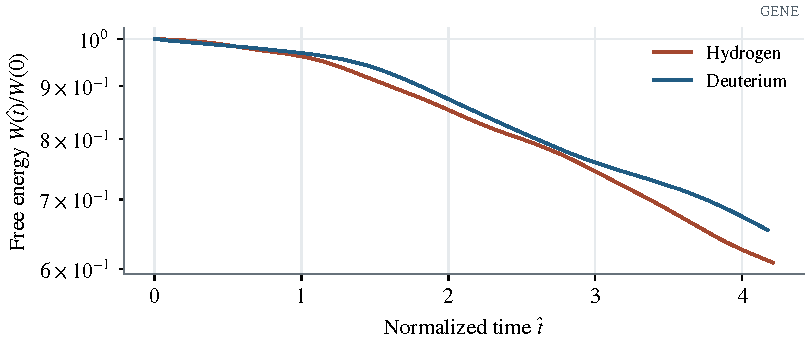
\includegraphics[width=.81\linewidth]{05_zero_gradient_energy.pdf}
\caption{Dimensionless free energy $W/W(0)$ versus normalized time $\ttime$ for the hydrogen and deuterium zero-gradient IV records at $\kn=0.7$. The energy decreases in both observed histories. A signed frequency or converged eigenmode cannot be inferred from these curves.}\label{fig:zero}\end{figure}

At fixed common gradients of 2, growth falls as $k_y$ increases and real frequency increases in the five qualified isotope pairs from 0.5 to 2 (Fig.~\ref{fig:isowave}). Hydrogen grows faster at each common sample. These points establish the ordering over a sampled wavelength interval, with no general assertion about smaller $k_y$.

\studyfig{06_isotope_wavenumber}{fig:isowave}{Hydrogen and deuterium wavenumber comparison at common $\omn=\omt=2$. The left panel gives growth and the right gives real frequency in GENE units. The horizontal value measures binormal scale, with larger values corresponding to shorter binormal wavelengths.}

\section{Phase 2: density gradients in electron--deuterium}
The density study holds $\omt_e=\omt_D=2$. At every common density gradient sampled between $\kn=0.5$ and 1.5, the growth rate falls and the positive real frequency increases with wavenumber (Fig.~\ref{fig:wavenumber}). At a fixed sampled wavenumber, increasing the common gradient raises both rates. At $\kn=0.7$ the qualified density range is 0.5 to 5, with growth increasing from 2.685 to 5.934 and real frequency from $+0.401$ to $+1.986$. Growth increases more slowly at larger gradients, whereas frequency is close to linear over these points (Fig.~\ref{fig:density}). Neither the most unstable wavenumber over the entire spectrum nor the onset density gradient has been located. The common density trend describes the joint equilibrium change.

\studyfig{10_deuterium_wavenumber}{fig:wavenumber}{Two-species deuterium study at $\omt_e=\omt_D=2$. Color identifies the common density gradient in both panels. Points are converged IV samples; the connecting lines guide the eye. The $\kn=0.3$ point at common $\omn=2$ is the qualified 32-point half-step result, checked against the 48-point control in Appendix~\ref{app:lowky}.}
\studyfig{11_deuterium_density}{fig:density}{Two-species deuterium growth and real frequency versus the common density gradient at fixed $\omt_e=\omt_D=2$. Curves at different fixed wavenumbers have the same color in both panels. The wider gradient range belongs to $\kn=0.7$.}

\subsection{What the potential profile adds}
The complex potential is the Fourier amplitude of the electrostatic perturbation along one field line. The coordinate $s/L_{\rm tube}$ is position along the traced turn divided by its length. The peak-normalized envelope $|\phi(s)|/\max_s|\phi(s)|$ compares spatial patterns independent of overall amplitude. The phase of an eigenmode has an arbitrary global offset. We rotate each complex profile to maximize its overlap with the reference and set the reference phase at the first node to zero. Spatial phase describes relative phase between positions at a fixed time. Real frequency comes from the \emph{temporal} phase slope in Eq.~\eqref{eq:mode}.

Figure~\ref{fig:modes} shows a similar overall envelope across the common gradient and wavenumber families, with a changing depression near the middle of the plotted field line. Complex overlap with the central case exceeds 0.9992 in the original nine-point matrix and is 0.9946--0.9984 for the higher-wavenumber additions. This supports a related spatial pattern throughout the measured band. Overlap alone leaves the number of branches and their driving mechanisms undetermined. The relative spatial-phase comparison is in Appendix~\ref{app:evidence}.

\studyfig{12_mode_amplitude}{fig:modes}{Peak-normalized deuterium potential along the field line at $\omt_e=\omt_D=2$. Left: common density-gradients at fixed $\kn=0.7$. Right: wavenumber variation at common $\omn=2$. These are parallel profiles of binormal Fourier components; \texttt{kymin} is a binormal wavenumber.}

\subsection{A charge-balanced electron-gradient path}
For two species with charges $-e$ and $+e$, $n_e=n_D$ must hold as an equilibrium profile and therefore $\omn_e=\omn_D$. Holding the deuterium density gradient fixed while changing the electron gradient requires a third charged population or a new equilibrium model. With fully ionized helium,
\begin{equation}
 n_e=n_D+2n_{\rm He},\qquad
 f=\frac{2 n_{\rm He}}{n_e},\qquad
 \omn_e=(1-f)\omn_D+f\omn_{\rm He}.
 \label{eq:neutrality}
\end{equation}
Here $f$ describes the helium positive-charge fraction at the reference surface. Positive profiles that satisfy the balance locally can be constructed by prescribing deuterium and helium exponentials with the intended scale lengths and setting $n_e(x)=n_D(x)+2n_{\rm He}(x)$. Their derivatives yield Eq.~\eqref{eq:neutrality}. The fraction may vary radially within each equilibrium even though its reference value is identical across the pilot. This is a local prescribed-profile model in the imposed ring field, with no global pressure-balance reconstruction.

GENE accepts multiple kinetic ion species, normalizes the input densities to the electron density, and checks both charge density and its charge-weighted equilibrium gradient. Its Landau collision implementation accepts the three active species. We used charges $(-1,+1,+2)$, masses $(0.00054462,2,4)$ in proton mass units, and densities $(1,0.75,0.125)$. All reference temperatures and temperature gradients are equal across species ($T_s/T_{\rm ref}=1$, $\omt_s=2$). Thus $Z_{\rm eff}=\sum_i n_i Z_i^2/n_e=1.25$ at the reference surface. With $\omn_D=2$ and $f=0.25$, we paired $\omn_e=1.75,2,2.25$ with $\omn_{\rm He}=1,2,3$. These choices avoid reversed or extreme helium gradients; at this fraction an electron gradient below 1.5 would require a hollow local helium profile. The midpoint is the matched three-species baseline.

\HeliumResult

\studyfig{15_compensated_electron_gradient}{fig:helium}{Compensated electron-gradient pilot with three kinetic species at $\kn=0.7$, $f=0.25$, $\omt_s=2$ and $\omn_D=2$. The three electron gradients require helium gradients 1, 2 and 3, respectively. The central sample is the matched three-species reference.}

Any change in the plotted rates measures the response along a path in which both electron and helium gradients vary. It does not yield the partial derivative with respect to the electron gradient at fixed helium gradient. Adding helium also changes the equilibrium species mix, ion polarization and collision terms relative to the two-species study. One possible companion path would fix $\omn_e=2$ and use $\omn_D=(1.75,2,2.25)$ with $\omn_{\rm He}=(2.75,2,1.25)$ at unchanged $f=0.25$. That proposal varies deuterium together with compensating helium and was outside this pilot.

\section{Kinetic versus adiabatic electrons}
The adiabatic-electron approximation assumes that electrons adjust rapidly along the field and give an approximately isothermal density response. A positive electrostatic potential attracts them. For a perturbation $\phi_1$, the Boltzmann relation is
\begin{equation}
 \frac{\delta n_e}{n_{0e}}=\frac{e}{T_e}\bigl(\phi_1-\langle\phi_1\rangle_{\rm FS}\bigr).
\end{equation}
The flux-surface mean vanishes for our nonzonal component. Thus the perturbation drives a density response in phase with the potential. Kinetic electrons instead have an evolving distribution, including trapped-particle motion, drift resonances and phase mixing. Removing those dynamics changes the field coupling and can alter both driving and damping. GENE retains kinetic ions in both runs \cite{plunk2014,goerler2011}.

At common gradients of 2 and $\kn=0.7$, both collisionless IV treatments on the $24\times48\times24$ grid converged. The kinetic case gave $(\gr,\fr)=(4.176,+0.944)$ and the adiabatic case gave $(0.136,-0.029)$, a 96.7\% reduction in growth (Fig.~\ref{fig:closure}). The adiabatic rate is still positive, so that mode is unstable. The phase rotates in the opposite sense under Eq.~\eqref{eq:mode}, and the amplitude now peaks near the middle of the plotted turn. The approximate pre-recurrence fit $(0.13613,-0.02939)$ agrees with the final fit $(0.13595,-0.02942)$. The result shows strong sensitivity to the electron model. It does not isolate a unique kinetic drive or establish that the two closures selected the same branch. The small adiabatic frequency still merits a common-timestep, velocity-resolution and recurrence check.

\studyfig{13_electron_response}{fig:closure}{Matched collisionless deuterium comparison at common gradients of 2 and $\kn=0.7$. Top: native growth and real frequency. Bottom: peak-normalized shape along the field line. Replacing kinetic electrons by the Boltzmann response weakens the instability and reverses temporal phase rotation.}

\section{Numerical confidence and remaining questions}
\subsection{Reference-grid comparison}
For the reference deuterium point at common gradients of 2 and $\kn=0.7$, the economical grid has nearly the same rates as the original grid and took about half as long (Table~\ref{tab:reference}). The original discretization is a numerical comparator, with no exact analytical rate available. For any rate $q$, the relative difference is $100|q_{\rm econ}-q_{\rm orig}|/|q_{\rm orig}|$ percent. The 1\% threshold is an adopted exploratory screen for this study. The moment-domain sensitivity shows why passing that screen for one pair of grids does not establish accuracy across all numerical options.

\begin{table}[H]\centering\small
\caption{Reference-grid comparison. Parentheses give the native reported rates. Other rates come from a shared late-time fit interval. Time is recorded GENE wall time, in seconds.}\label{tab:reference}
\begin{tabular}{@{}lccc@{}}\toprule
Grid $(n_z,n_v,n_\mu)$ & Growth $\gr$ & Real frequency $\fr$ & Wall time (s) \\\midrule
Original $32\times48\times32$ & 4.171900 (4.172) & 0.946175 (0.946) & 232.111 \\
Economical $24\times48\times24$ & 4.178982 (4.179) & 0.946787 (0.947) & 111.678 \\
Absolute relative difference & 0.170\% & 0.065\% & 51.9\% less \\
\bottomrule\end{tabular}
\end{table}

With matched timestep, increasing the magnetic-moment extent from 12.25 to 16.25 changed fitted real frequency by 4.93\%. A quadrature refinement in the wider domain left a 4.90\% difference from the nominal domain. This is a reference-point sensitivity to the numerical velocity domain. It is not an uncertainty common to all cases. Appendix~\ref{app:numerical} retains the timestep, parallel-grid and velocity-grid checks.

\subsection{The low-wavenumber question}
\LowKyResult

A longer binormal wavelength changes ion gyroaveraging, drift frequencies and the balance of kinetic response. The resulting change in stability need not be monotone. A converged exponential increase with a settled smooth shape supports a growing mode; a finite transient or an apparent decay provides weaker evidence. Establishing a change of branch requires a reproducible competing spatial and temporal signature.

\section{Conclusions}
The pair benchmark separates instability from phase rotation. The two-species kinetic studies establish an isotope ordering and a common-density and binormal-scale dependence across qualified samples. The helium pilot tests a feasible equilibrium path and shows what can be varied while keeping the deuterium gradient fixed. At one matched collisionless operating point, dynamical electrons strongly change the deuterium instability. A resolved peak or threshold would need qualified sampling outside the present ranges. The weak adiabatic mode and the physical interpretation of the electron and helium sensitivities require further targeted work.

\clearpage
\appendix
\section{Numerical settings and supporting diagnostics}\label{app:numerical}
GENE 3.1 patch 5 at source revision \texttt{a0d2f213} was used in double precision on Apple Silicon. The original installation passed 126 diagnostic comparisons in 11 selected tests. The project data are organized by exact input and diagnostic hash in the report package. We retain the IV format and solver settings in all follow-up runs.

\begin{table}[H]\centering\small
\caption{Baseline numerical settings. Configuration files give exact case-specific values.}
\begin{tabular}{@{}lp{.65\linewidth}@{}}\toprule
Quantity & Value \\\midrule
Electrostatic limits & $\beta=0$, \texttt{debye2 = 0}; local imposed ring dipole \\
Grid & Original $32\times48\times32$, economical $24\times48\times24$ \\
Velocity extents & $L_v=3.5$, $L_\mu=12.25$ nominal, $L_\mu=16.25$ in domain tests \\
Time stepping & RK4 with automatic choice or documented fixed-step controls \\
Species & Equal-mass pair reference; isotope runs have $m_e=0.00054462$, $m_H=1$, $m_D=2$ in proton units \\
Density and temperature & Equal densities and reference temperatures for the two-species scans. Eq.~\eqref{eq:neutrality} for the helium pilot. \\
\bottomrule\end{tabular}
\end{table}

At fixed reference physics, comparing 32 and 64 parallel nodes gave 4.172 and 4.163 in native growth and the same printed frequency, 0.946. A matched step at 32 points isolated a negligible rate change. The 24-point parallel run retained good agreement at that matched step. Separate $v_\parallel$ and $\mu$ refinements and the combined-grid checks are summarized in Fig.~\ref{fig:resolution}. In contrast, the $n_v=32$ automatic step and wider magnetic-moment domain produced runaway behavior in their original automatic schedules. A smaller fixed step stabilized both configurations. Figure~\ref{fig:domain} shows that a width-dependent frequency shift remained at matched timestep.

\studyfig{07_resolution_and_timestep}{fig:resolution}{Reference-point changes of common-window growth and real-frequency fits for controlled grid and timestep comparisons. Values are relative to each comparator on a logarithmic percent axis. The dashed 1\% screen is a working criterion for the exploratory reference.}
\studyfig{08_velocity_and_domain_controls}{fig:domain}{Top: normalized free energy for fixed and automatic schedule checks at coarse $v_\parallel$ resolution and with widened magnetic-moment extent. Bottom: fitted growth and real frequency for nominal and wider domains at a fixed timestep. The wider-domain quadrature change leaves most of the frequency shift intact.}
\studyfig{14_reference_field_settling}{fig:settling}{Reference deuterium diagnostics at $\kn=0.7$ and common gradients of 2. Left: the time-window phase slope approaches the native real frequency. Right: one minus each run's normalized complex overlap with its own final profile. The small ripples support comparing rates on matched fit windows.}
\FloatBarrier

\section{Qualification of the \texorpdfstring{$\kn=0.3$}{kymin = 0.3} records}\label{app:lowky}
The original $32\times48\times32$ run applied $\Delta\ttime=0.000835$, advanced 3129 reported steps, and reached $\ttime=2.61355$. It printed $\gr=378.519$ and $\fr=+220.647$ and recorded 29 amplitude rescalings. The saved field itself shows 29 corresponding abrupt decreases. A rescaling multiplies a linear perturbation by a common factor to keep the arithmetic in range; the jumps do not represent physical changes in plasma energy. Likewise, rescales alone do not disqualify a run. Here the raw terminal field changes sharply between neighboring nodes, and its complex overlap with the conservative $\kn=0.5$ reference is 0.00156. The adjacent-node norm $\|\Delta_s\phi_0\|_2/\|\phi_0\|_2$ is 1.556, compared with 0.00464 at 0.5.

The ten-step native log-ratio applies a principal complex logarithm. At diagnostic interval $10\Delta\ttime$, it measures phase modulo $2\pi$. Per-step unwrapping gives about $-2036.82$ in the final uninterrupted segment. Applying the native spatial weights on the exact ten-step diagnostic window gives $-2036.7853$ before wrapping. Adding three frequency alias intervals $2\pi/(10\Delta\ttime)$ gives $+220.6466$. Reapplying the native amplitude-weighted ten-step log-ratio to the final raw field gives $(378.5190,+220.6466)$. This reproduces the native diagnostic and reveals frequency aliasing of the rapidly changing field. Even the per-step value describes that recorded discrete signal, with no claim about a physical mode. The growth slope itself is large over the terminating segment, so fixing frequency interpretation alone does not resolve the run.

\LowKyDetails

\begin{table}[H]\centering\small
\caption{Two-species $\kn=0.3$ audit at common gradients of 2. All rows carry a native flag. The original rates are unresolved. The two fixed-step runs qualify on the tested grids.}
\begin{tabular}{@{}lrrrrrr@{}}\toprule
Setup & $n_z$ & $\Delta\ttime$ & Steps & Native $\gr$ & Native $\fr$ & Rescales \\
\midrule
\LowKyRows
\bottomrule\end{tabular}
\end{table}

\studyfig{16_low_wavenumber_controls}{fig:lowky}{Two-species deuterium at $\kn=0.3$, common $\omn=\omt=2$. The panels show the recorded normalized free energy and the final peak-normalized spatial envelope. The automatic run is the original anomalous case. The other curves are the documented fixed-step comparisons. Abrupt energy resets in the original diagnostic are numerical amplitude rescalings.}
\FloatBarrier

\section{Historical qualification, spatial phase and reproducibility}\label{app:evidence}
The five pair extensions from the historical joint-gradient survey yielded two underflow stops and three step-limit stops. In Fig.~\ref{fig:pairenergy}, decay and apparent amplification alone leave the temporal and spatial qualification incomplete. Two traces contain amplitude renormalizations. They are treated as numerical bookkeeping rather than physical energy loss. These records supply no qualified complex rates.

\studyfig{03_pair_unresolved_energy}{fig:pairenergy}{Free-energy diagnostics for the extended historical pair IV cases at $\kn=0.7$. Each label gives $(\omn,\omt)$ and each trace uses its own initial energy. The resets occur when the code renormalizes the perturbation. None of the five runs provides a qualified complex modal rate.}

The 13 isotope energy estimates were checked over the final 50\%, 30\% and 15\% of stored samples. The historical screen used $R^2>0.99$ for the two shorter windows and required maximum growth-slope drift below $\max(0.05,0.1|\gr_{15}|)$. Five passed. The uniform deuterium finite-time decay estimate was qualified separately because its slopes agreed and the 30\% $R^2=0.9894$ narrowly missed the screen. These six estimates are kept separate from the 85 native converged results, and seven estimates remain uncertain. The two illustrated cases in Fig.~\ref{fig:fit} demonstrate why a good fit to one narrow window alone is insufficient.

\studyfig{05_isotope_fit_examples}{fig:fit}{Historical deuterium energy estimates at $\kn=0.7$ and $\omn=0$. Brown dashed segments show fits over the final 15\% of saved samples. The $\omt=1$ estimate is uncertain because the slope varies with fit interval. These plots estimate growth only.}
\studyfig{12_mode_phase}{fig:spatialphase}{Relative spatial phase for the same qualified profiles as Fig.~\ref{fig:modes}. Each field is aligned by a single phase offset to the common reference. These variations describe phase differences across position at a fixed time. A temporal phase slope, rather than this spatial variation, supplies the real frequency.}
\FloatBarrier

\begin{table}[H]\centering\small
\caption{Qualified Phase 2 two-species rate pairs. Both temperature gradients are 2. The separately qualified half-step point at $\kn=0.3$ is tabulated in Appendix~\ref{app:lowky}.}
\begin{tabular}{@{}rrrcl@{}}\toprule
Common $\omn$ & $\kn$ & $\gr$ & $\fr$ & Grid\\\midrule
\matrixrows
\bottomrule\end{tabular}
\end{table}

\begin{table}[H]\centering\small
\caption{Finite-time free-energy results for all 13 unresolved Phase 1 isotope points. Windows use the final 50\%, 30\%, and 15\% of sampled times. These estimates supply no real frequency.}
\begin{tabular}{@{}lrrcccl@{}}\toprule
Isotope & $\omn$ & $\omt$ & $\gr_{50}$ & $\gr_{30}$ & $\gr_{15}$ & Quality\\\midrule
\energyfitrows
\bottomrule\end{tabular}
\end{table}

The \href{https://github.com/santoshzaero/gene-dipole-plasma-stability}{research repository} preserves the full input files, curated raw-output hashes, historical results and benchmark. The report package contains the figures, numerical tables, extraction scripts and a figure-to-data inventory. The package README gives the offline figure and LaTeX build commands.
\FloatBarrier
\bibliographystyle{unsrt}
\bibliography{references}
\end{document}
